%!TEX root = ../main.tex
\newcommand{\vcenteredinclude}[1]{\begingroup
\setbox0=\hbox{\includegraphics[width = 0.3\textwidth]{#1}}%
\parbox{\wd0}{\box0}\endgroup}

\begin{frame}{Algorithmes évolutionnistes}
   \textbf{Algorithmes évolutionnistes (AE)}\\
  \textit{Type : }Métaheuristique\\
  \textit{Stochastique : } Oui\\
  \textit{Caractéristique : } Évolution d'une population de solutions
  \vspace{0.5cm}
  \hrule
\vspace{0.2cm}
\textbf{Principes}\\
1. Chaque solution possède un niveau \textit{d'adaptation} \\
2. Opérateurs de \textit{variation} pour générer de nouvelles solutions  \\
3. Opérateurs de \textit{sélection} pour améliorer l'adaptation des solutions
\end{frame}

\begin{frame}{Schéma d'un AE}
	\begin{figure}[tb]
    	\centering
    	\includegraphics<1>[width=0.95\textwidth]{figures/cycle_evolution.pdf}
	\end{figure} 
\end{frame}


% \begin{frame}{Caractéristiques des AE}
	
% \begin{figure}[tb]
%     \centering
%     \includegraphics<1>[width=0.95\textwidth]{figures/triforce.pdf}
% \end{figure} 
% \end{frame}

\begin{frame}{Problème du sac à dos}
\textbf{Knapsack problem}\\
Un revendeur de chocolat doit distribuer sa précieuse cargaison et récolter ses gains. Malheureusement, il n'a le temps de faire qu'une seule tournée avant que son fournisseur n'arrive et son sac à dos peut transporter au plus une masse $M$. \\
\textit{Quel est le sous-ensemble d'objets lui permettant de garder ses deux jambes?}
  
\begin{figure}[tb]
    \centering
    \includegraphics<1>[width=0.85\textwidth]{figures/knapsack.pdf}
\end{figure} 
\end{frame}

\begin{frame}{Implémentation d'un algorithme génétique}
\begin{itemize}
  \item \textbf{Représentation du génome : } \vcenteredinclude{figures/bitString.pdf}
  \item \textbf{Niveau d'adaptation :} Prix total des objets sélectionnés 
  \item \textbf{Sélection des parents : } Tournoi
  \item \textbf{Croisement des parents : } \\ \vspace{5pt}
  \includegraphics<1>[width=0.85\textwidth]{figures/croisement.pdf}
  \item \textbf{Mutation :} \\ \vspace{5pt}
  \includegraphics<1>[width=0.85\textwidth]{figures/mutation.pdf}
\end{itemize}
  
\end{frame}

\begin{frame}{Problème du sac à dos - Distribution du génome}
  Vidéo
\end{frame}

\begin{frame}{Problème du sac à dos - Adaptation}
\vspace{-10pt}
\textbf{Niveau d'adaptation des populations}
  \begin{figure}[h!]
    \centering
    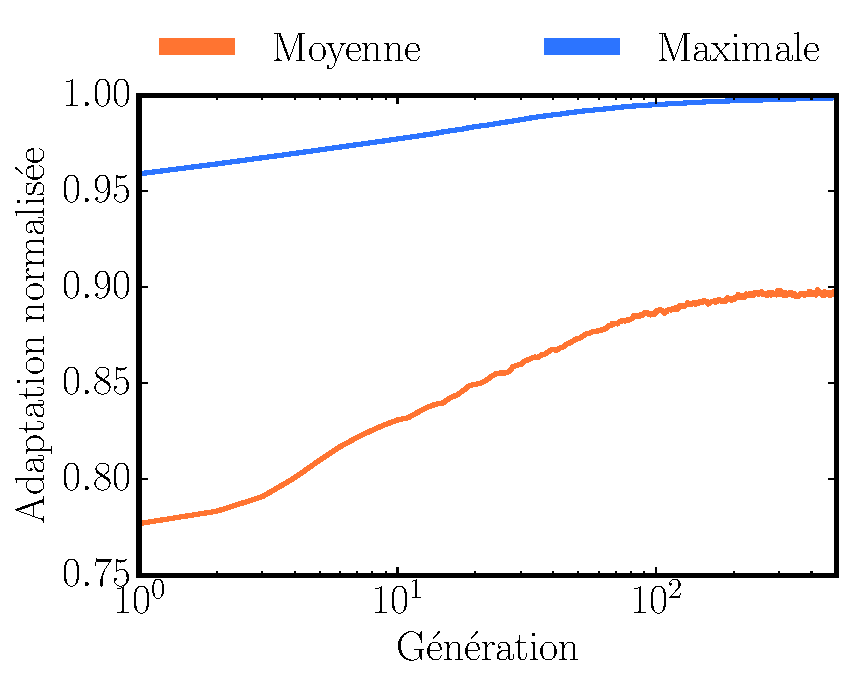
\includegraphics[width=0.75\textwidth]{figures/knapsack_adaptation.pdf}
  \end{figure}
\end{frame}